
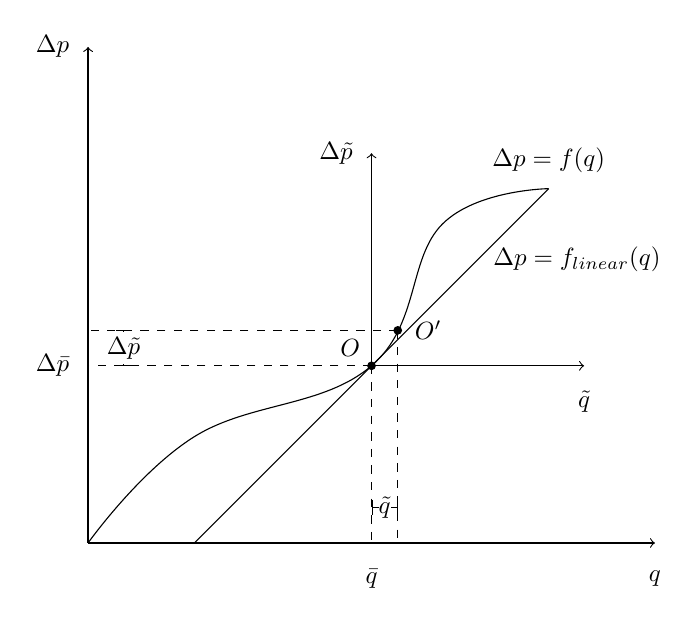
\begin{tikzpicture} [scale=0.9,transform shape]

\usetikzlibrary{decorations.markings}

  \draw[|-|] (5.87,-11) --
        node[fill=white,font=\normalsize,inner ysep=2pt,inner
                xsep=0]{$\tilde{q}$}(5.5,-11);
                
 \draw[|-|] (2,-9) --
        node[fill=white,font=\normalsize,inner ysep=2pt,inner
                xsep=0]{$\Delta \tilde{p}$}(2,-8.5);
\node at (5.2,-8.75) {$O$};
\node at (6.3,-8.5) {$O'$};
\node at (1,-4.5) {$\Delta p$};
\node at (8,-6.1) {$\Delta p = f(q)$};
\node at (8.4,-7.5) {$\Delta p = f_{linear}(q)$};
\node at (1,-9) {$\Delta \bar{p}$};
\node at (9.5,-12) {$q$};
\node at (5.5,-12) {$\bar{q}$};
\node at (8.5,-9.5) {$\tilde{q}$};
\node at (5,-6) {$\Delta \tilde{p}$};
\draw [->](1.5,-11.5) -- (1.5,-4.5);
\draw [->](1.5,-11.5) -- (9.5,-11.5);
\draw  plot[smooth, tension=.7] coordinates {(1.5,-11.5) (3,-10) (5.5,-9) (6.5,-7) (8,-6.5)};

\draw [black,fill=black] (5.87,-8.5) node (v4) {} circle (.35ex);
\draw [black,fill=black] (5.5,-9) node (v4) {} circle (.35ex);
\draw [thin](8,-6.5) -- (3,-11.5);
\draw [dashed](5.5,-9) -- (5.5,-11.5);
\draw [dashed](5.5,-9) -- (1.5,-9);
\draw [dashed](5.87,-8.5) -- (5.87,-11.5);
\draw [dashed](5.87,-8.5) -- (1.5,-8.5);
\draw [->](5.5,-9) -- (5.5,-6);
\draw [->](5.5,-9) -- (8.5,-9);
\end{tikzpicture}